\documentclass[tikz,svgnames,border=5pt]{standalone}
\usepackage{fontspec}
\setmainfont{Source Serif 4}
\setsansfont{Source Sans 3}
\setmonofont{Source Code Pro}
\usetikzlibrary{calc, positioning, patterns}

\definecolor{colTrack}{HTML}{B266FF}
\definecolor{colSectorFill}{HTML}{D5E8D4}
\definecolor{colSectorStroke}{HTML}{82B366}
\definecolor{colGeoSectorFill}{HTML}{DAE8FC}
\definecolor{colGeoSectorStroke}{HTML}{6C8EBF}
\definecolor{colClusterFill}{HTML}{F0A30A}
\definecolor{colClusterStroke}{HTML}{BD7000}

\begin{document}
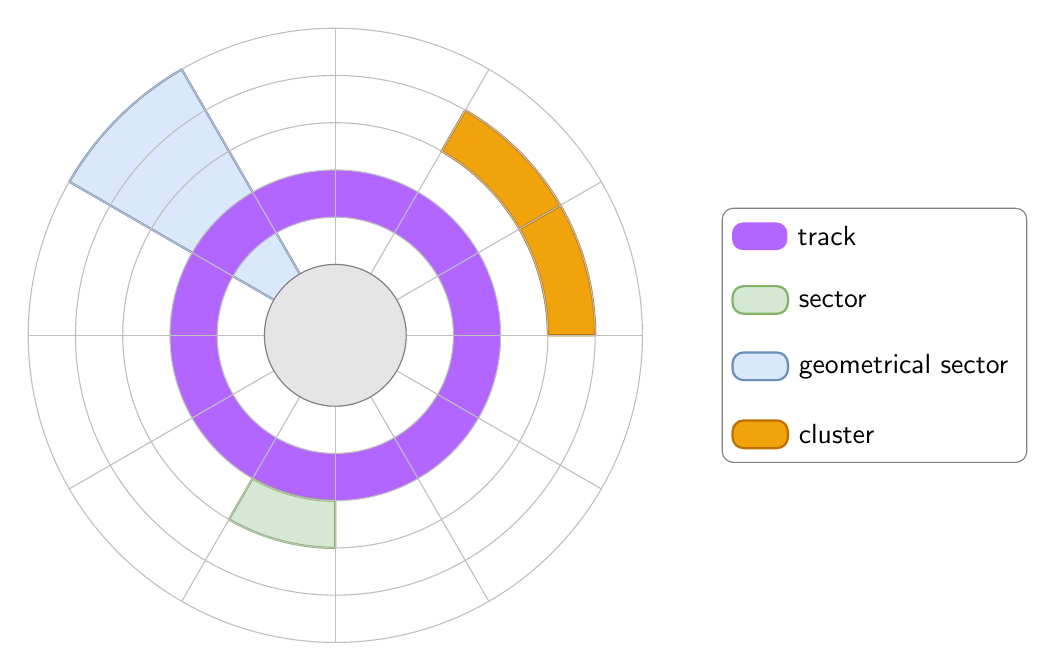
\begin{tikzpicture}[font=\sffamily]
  % Parameters
  \def\innerR{0.9}
  \def\trackWidth{0.6}
  \def\numTracks{5}
  \def\numSectors{12}
  \def\sectorAngle{360/\numSectors}

  % Draw Geometrical Sector (Blue) - Wedge
  % Spanning all tracks in one angular sector
  \fill[colGeoSectorFill] (0,0) -- (120:{\innerR+\numTracks*\trackWidth}) arc (120:150:{\innerR+\numTracks*\trackWidth}) -- cycle;
  \draw[colGeoSectorStroke, thick] (0,0) -- (120:{\innerR+\numTracks*\trackWidth}) arc (120:150:{\innerR+\numTracks*\trackWidth}) -- cycle;

  % Draw Track (Purple) - One full ring
  % Track 1 (innermost)
  \fill[colTrack, even odd rule] (0,0) circle ({\innerR+2*\trackWidth}) (0,0) circle ({\innerR+\trackWidth});

  % Re-draw the GeoSector part that was covered by the white fill of the track hole
  % Actually, the track is a ring. The GeoSector is a wedge.
  % If the track is purple, and GeoSector is blue, their intersection is interesting.
  % In the SVG, it seems they might be separate examples.
  % Let's put the Track highlight on a different ring than the Cluster/Sector if possible, or just let it be.
  % I'll highlight Track 1 (2nd from center).

  % Draw Cluster (Orange) - Group of sectors in a track
  % Track 3 (outermost), Sectors 0 and 1
  \foreach \s in {0,1} {
      \fill[colClusterFill] ({\s*\sectorAngle}:{\innerR+4*\trackWidth}) arc ({\s*\sectorAngle}:{(\s+1)*\sectorAngle}:{\innerR+4*\trackWidth}) -- ({(\s+1)*\sectorAngle}:{\innerR+3*\trackWidth}) arc ({(\s+1)*\sectorAngle}:{\s*\sectorAngle}:{\innerR+3*\trackWidth}) -- cycle;
      \draw[colClusterStroke, thick] ({\s*\sectorAngle}:{\innerR+4*\trackWidth}) arc ({\s*\sectorAngle}:{(\s+1)*\sectorAngle}:{\innerR+4*\trackWidth}) -- ({(\s+1)*\sectorAngle}:{\innerR+3*\trackWidth}) arc ({(\s+1)*\sectorAngle}:{\s*\sectorAngle}:{\innerR+3*\trackWidth}) -- cycle;
  }

  % Draw Single Sector (Green)
  % Track 2, Sector 8
  \fill[colSectorFill] (240:{\innerR+3*\trackWidth}) arc (240:270:{\innerR+3*\trackWidth}) -- (270:{\innerR+2*\trackWidth}) arc (270:240:{\innerR+2*\trackWidth}) -- cycle;
  \draw[colSectorStroke, thick] (240:{\innerR+3*\trackWidth}) arc (240:270:{\innerR+3*\trackWidth}) -- (270:{\innerR+2*\trackWidth}) arc (270:240:{\innerR+2*\trackWidth}) -- cycle;

  % Draw Grid Lines (on top of fills)
  \foreach \i in {0,...,\numTracks} {
    \draw[gray!50] (0,0) circle ({\innerR+\i*\trackWidth});
  }
  \foreach \i in {1,...,\numSectors} {
    \draw[gray!50] ({\i*\sectorAngle}:{\innerR}) -- ({\i*\sectorAngle}:{\innerR+\numTracks*\trackWidth});
  }

  % Center hole
  \fill[gray!20, draw=gray] (0,0) circle ({\innerR});

  % Legend
  \matrix [draw=black!50, rounded corners, fill=white, right=1cm of current bounding box.east, anchor=west, row sep=10pt, nodes={anchor=west}] {
    \node [rectangle, fill=colTrack, minimum width=2em, minimum height=1em, label=right:track] {}; \\
    \node [rectangle, fill=colSectorFill, draw=colSectorStroke, thick, minimum width=2em, minimum height=1em, label=right:sector] {}; \\
    \node [rectangle, fill=colGeoSectorFill, draw=colGeoSectorStroke, thick, minimum width=2em, minimum height=1em, label=right:geometrical sector] {}; \\
    \node [rectangle, fill=colClusterFill, draw=colClusterStroke, thick, minimum width=2em, minimum height=1em, label=right:cluster] {}; \\
  };
\end{tikzpicture}
\end{document}
